\chapter{Distribution of methylamine lines contaminated by other molecular line emission in Orion-KL
\label{chap:appendixA}}

\section{Integrated intensity maps}

%%%%% 積分強度図挿入 %%%%%
\begin{figure}[htbp] 
\begin{center}
\begin{minipage}{0.98\textwidth} 
\begin{center}
%%%% ここから
\begin{minipage}{0.48\textwidth}
\begin{center}
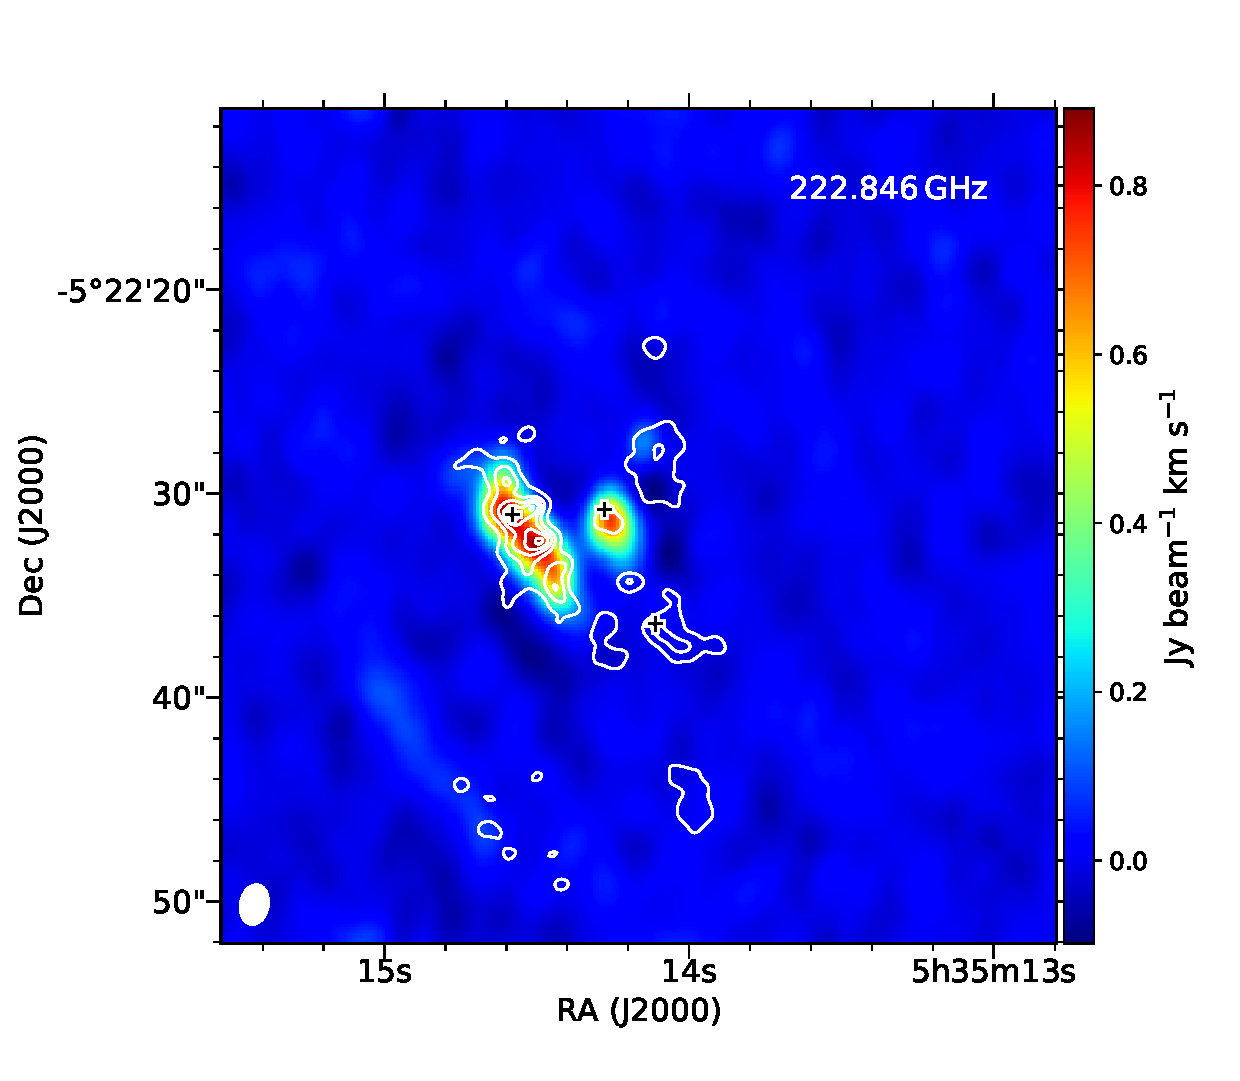
\includegraphics[width=0.98\textwidth]{OrionKL/mom0/222.846SV_mom0_3-7.eps}
%\\(a) 左の図の説明
\end{center}
\end{minipage}
\begin{minipage}{0.48\textwidth}
\begin{center}
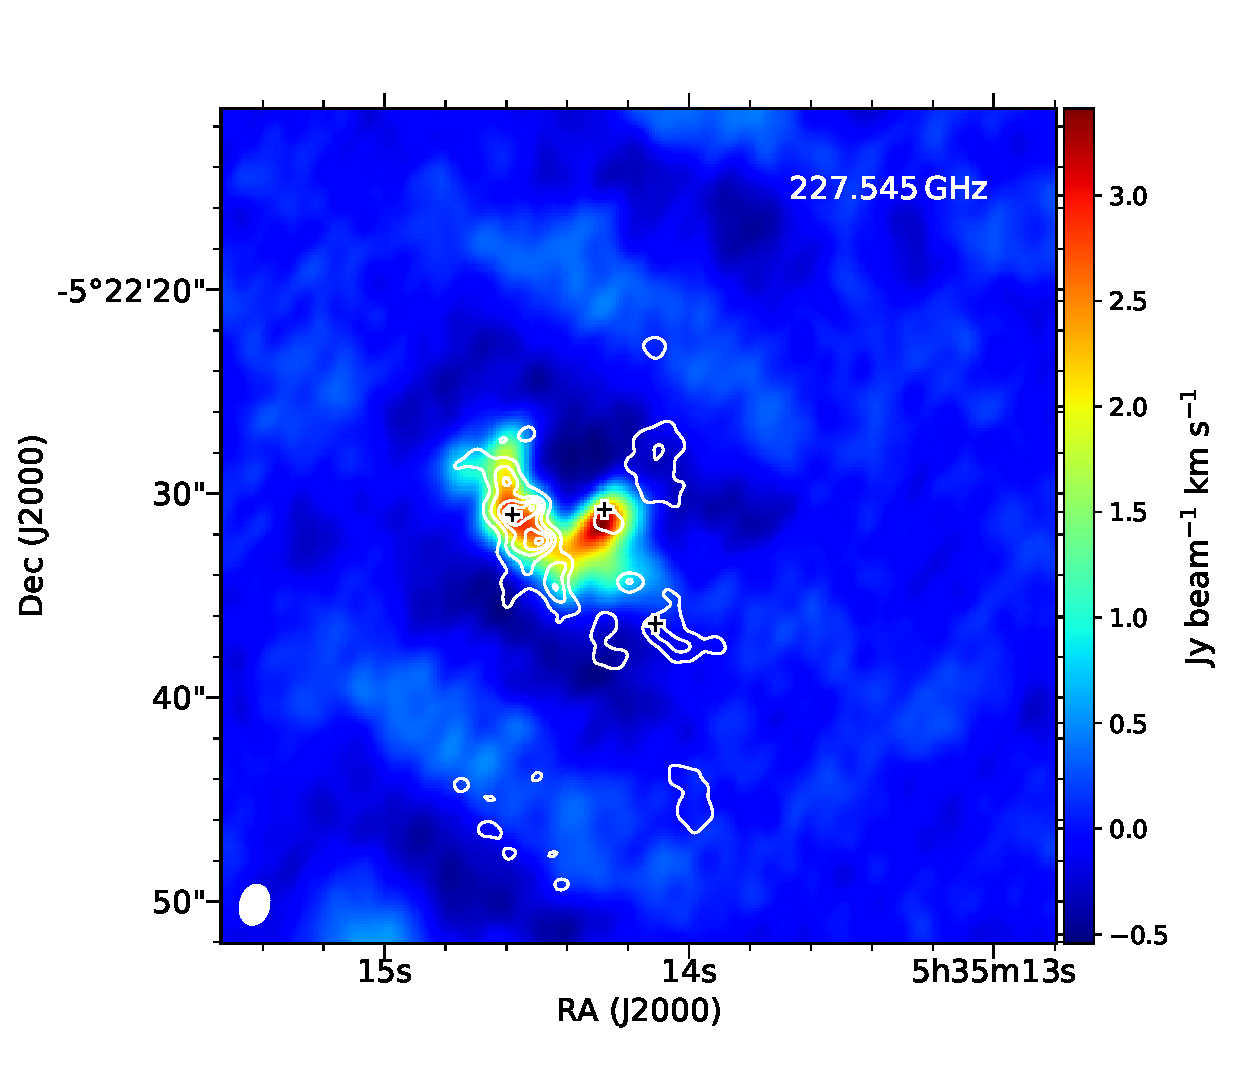
\includegraphics[width=0.98\textwidth]{OrionKL/mom0/227.545SV_mom0_3-7.eps}
%\\(b) 右の図の説明
\end{center}
\end{minipage}
\end{center}
\end{minipage}
%%%% ここまで一組

\begin{minipage}{0.98\textwidth} 
\begin{center}
\begin{minipage}{0.48\textwidth}
\begin{center}
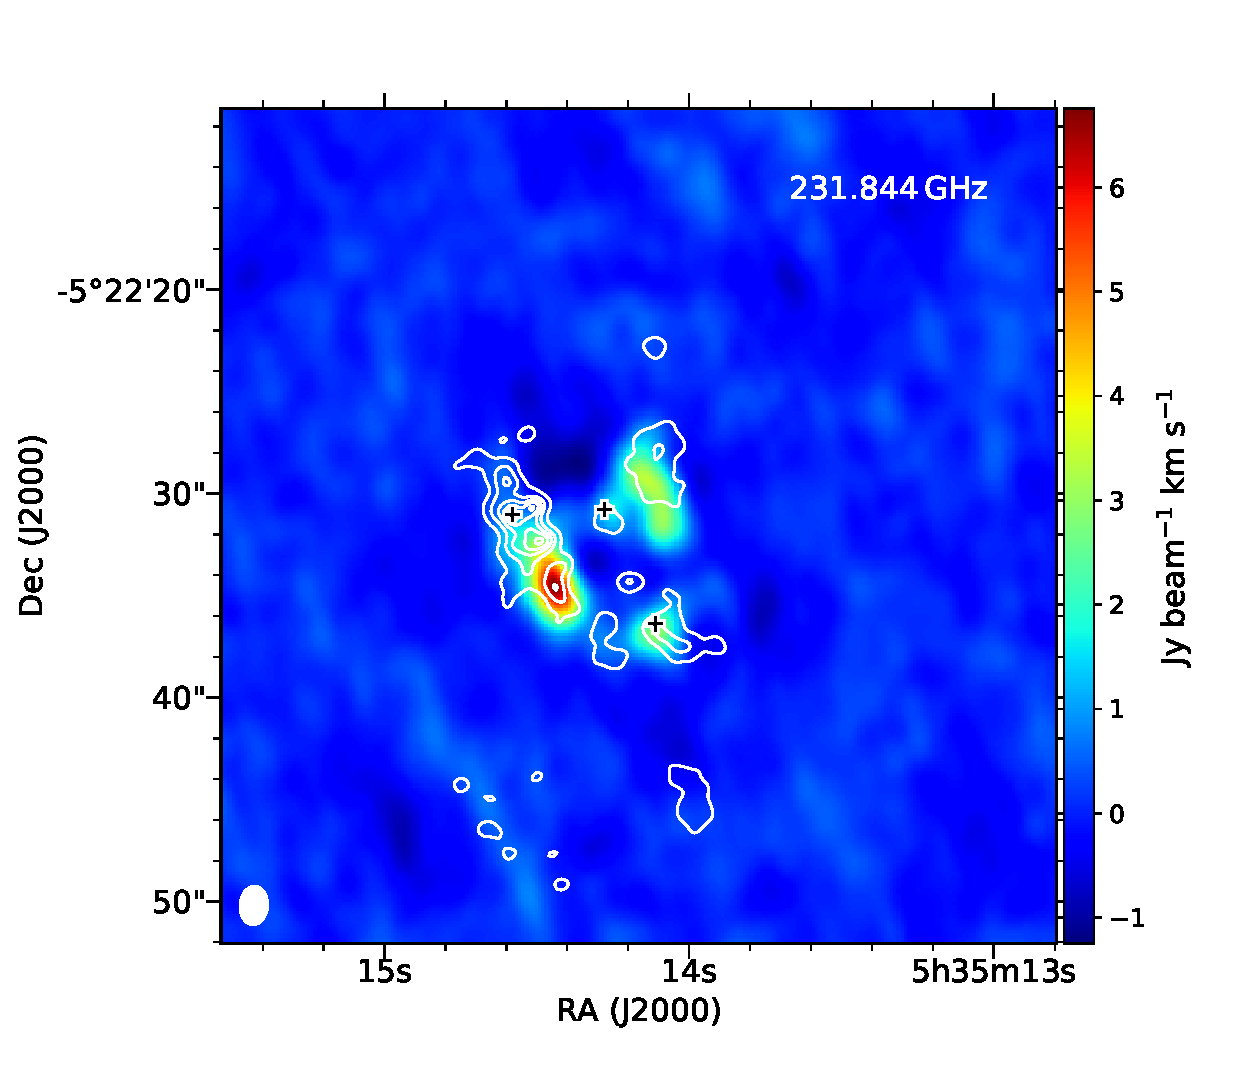
\includegraphics[width=0.98\textwidth]{OrionKL/mom0/231.844SV_mom0_3-7.eps}
%\\(c) 左の図の説明
\end{center}
\end{minipage}
\begin{minipage}{0.48\textwidth}
\begin{center}
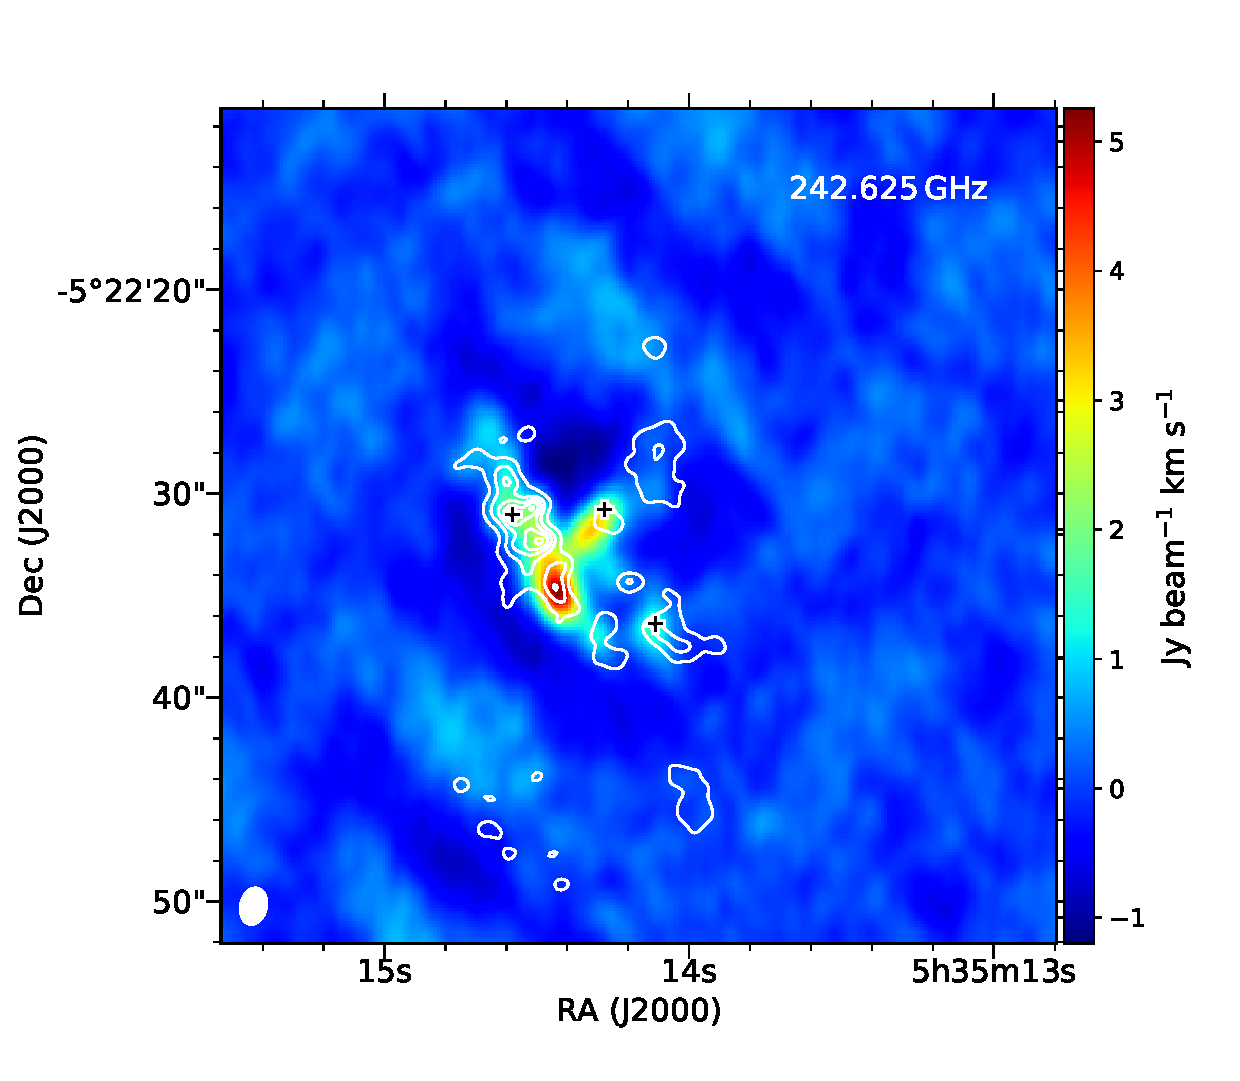
\includegraphics[width=0.98\textwidth]{OrionKL/mom0/242.625SV_mom0_3-7.eps}
%\\(d) 右の図の説明
\end{center}
\end{minipage}
\end{center}
\end{minipage}

\caption{Integrated intensity maps around methylamine line.}
\end{center}
\end{figure}

\newpage

%%%%% 積分強度図挿入 %%%%%
\begin{figure}[H] 
\begin{center}

%%%% ここから
\begin{minipage}{0.98\textwidth} 
\begin{center}
\begin{minipage}{0.48\textwidth}
\begin{center}
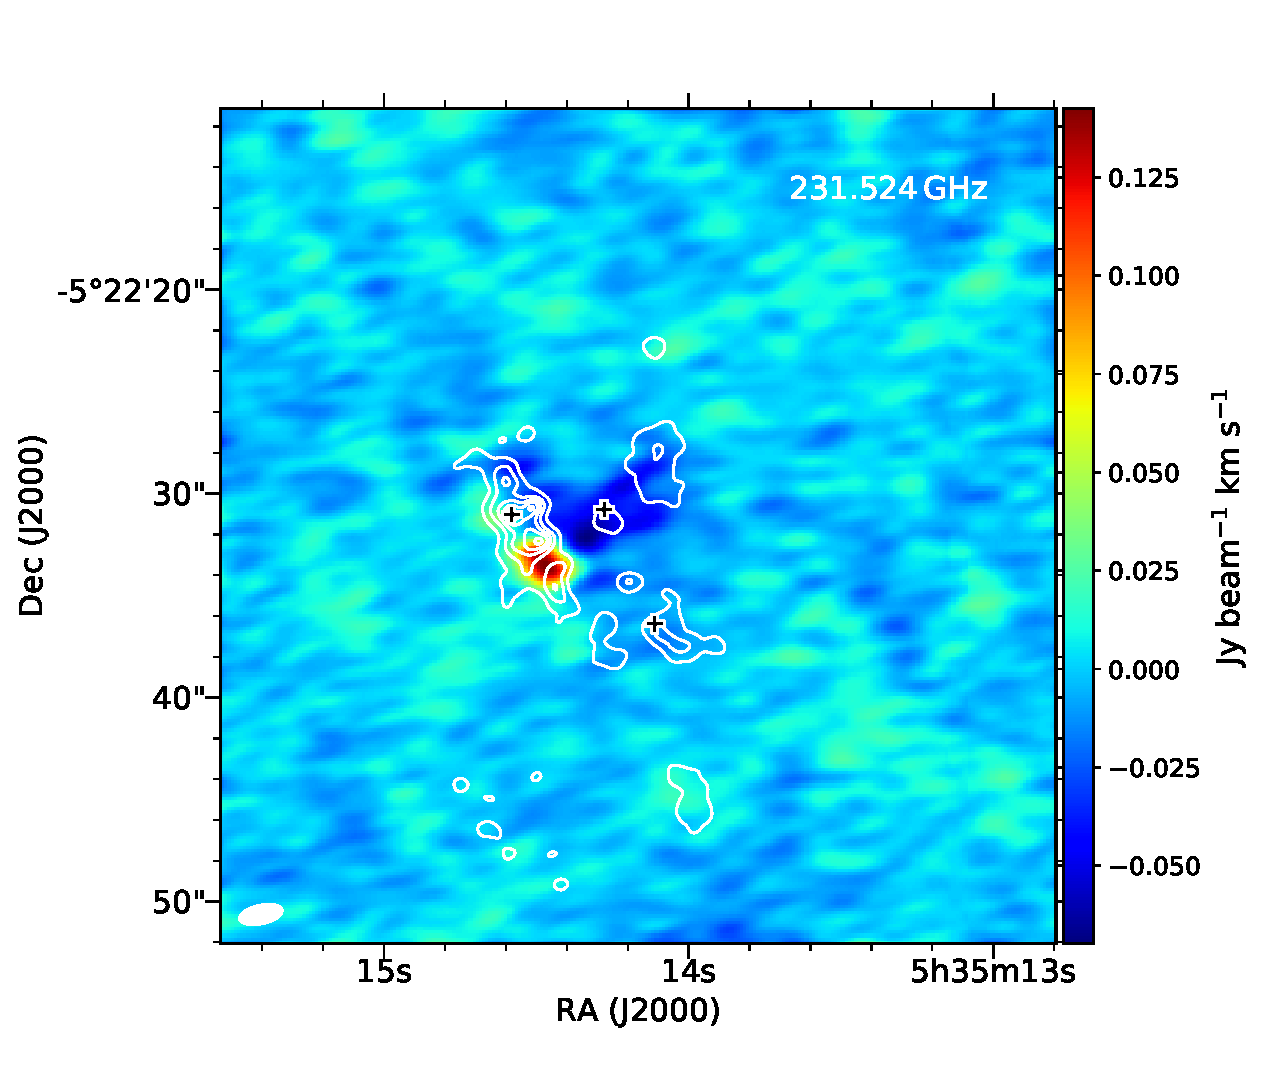
\includegraphics[width=0.98\textwidth]{OrionKL/mom0/231.524mom0_3-7.eps}
%\\(a) 左の図の説明
\end{center}
\end{minipage}
\begin{minipage}{0.48\textwidth}
\begin{center}
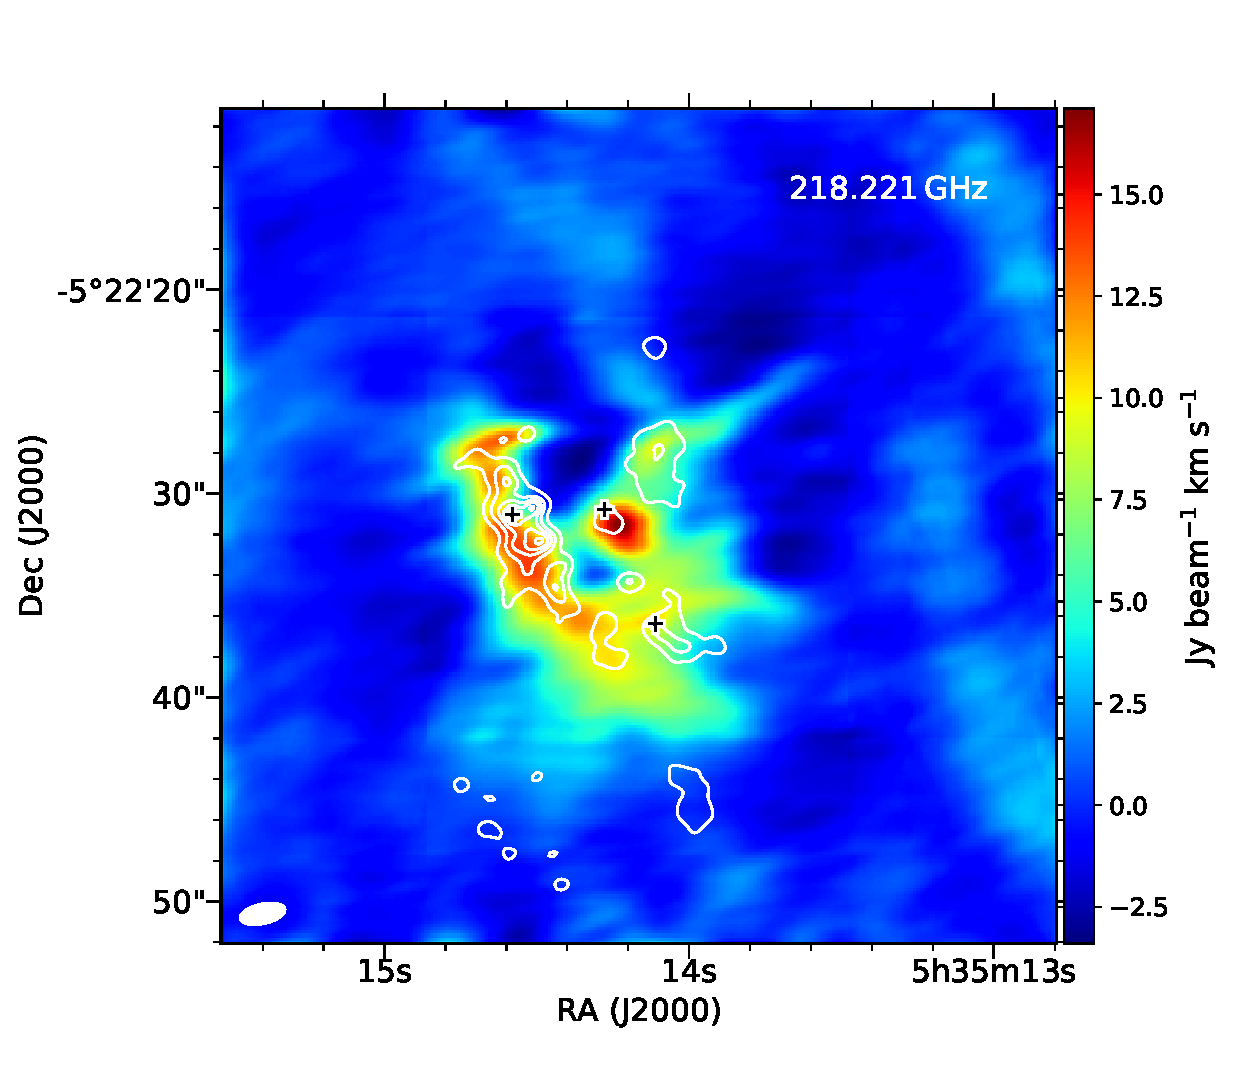
\includegraphics[width=0.98\textwidth]{OrionKL/mom0/218.221mom0_3-7.eps}
%\\(b) 右の図の説明
\end{center}
\end{minipage}
\end{center}
\end{minipage}
%%%% ここまで一組

\begin{minipage}{0.98\textwidth} 
\begin{center}
\begin{minipage}{0.48\textwidth}
\begin{center}
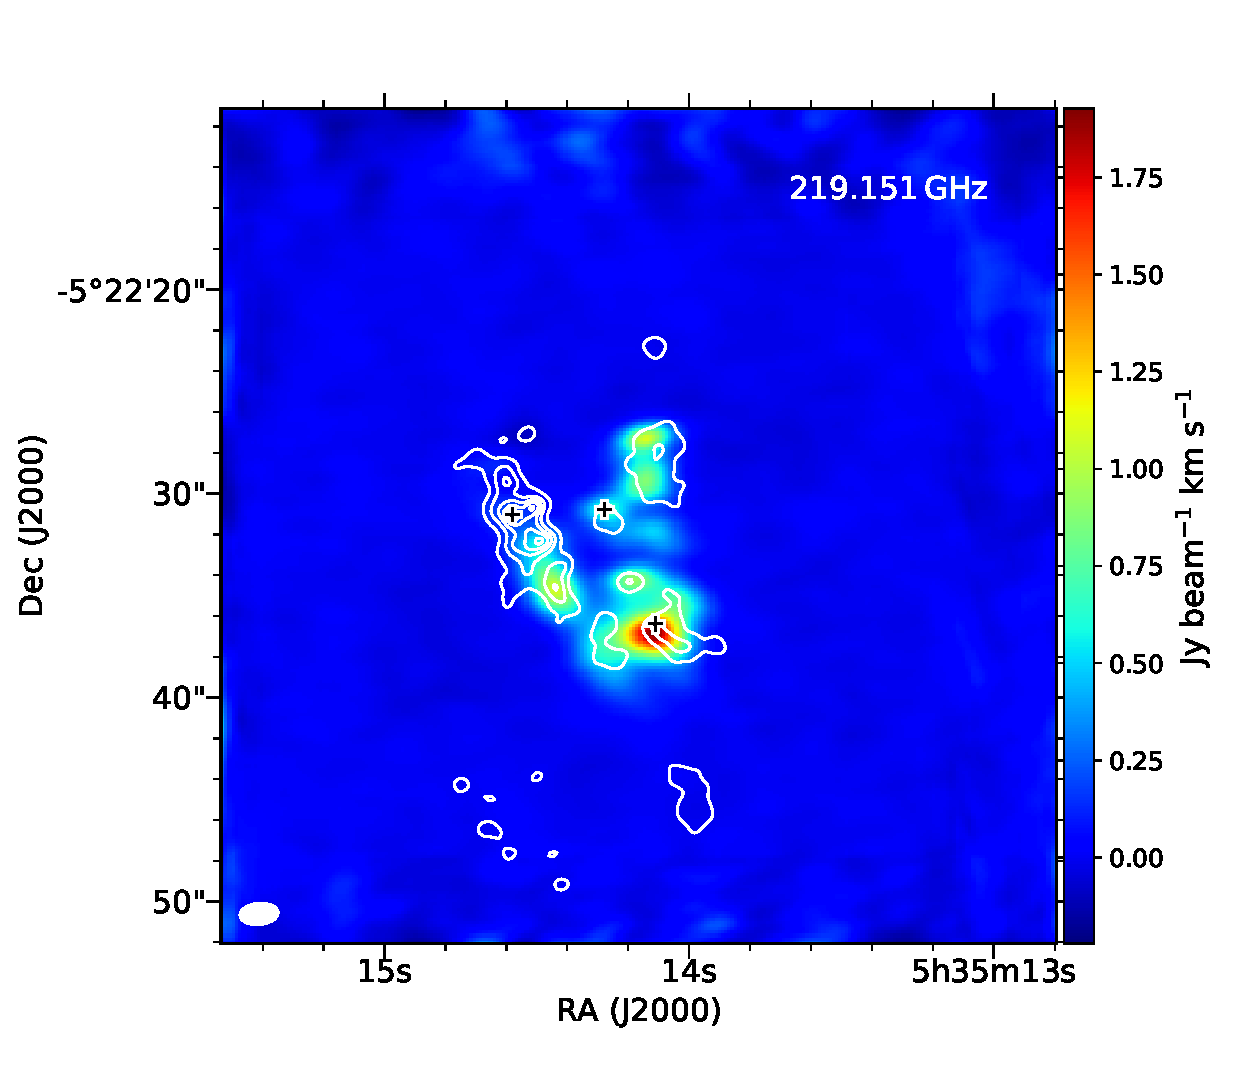
\includegraphics[width=0.98\textwidth]{OrionKL/mom0/219.151mom0_3-7.eps}
%\\(c) 左の図の説明
\end{center}
\end{minipage}
\begin{minipage}{0.48\textwidth}
\begin{center}
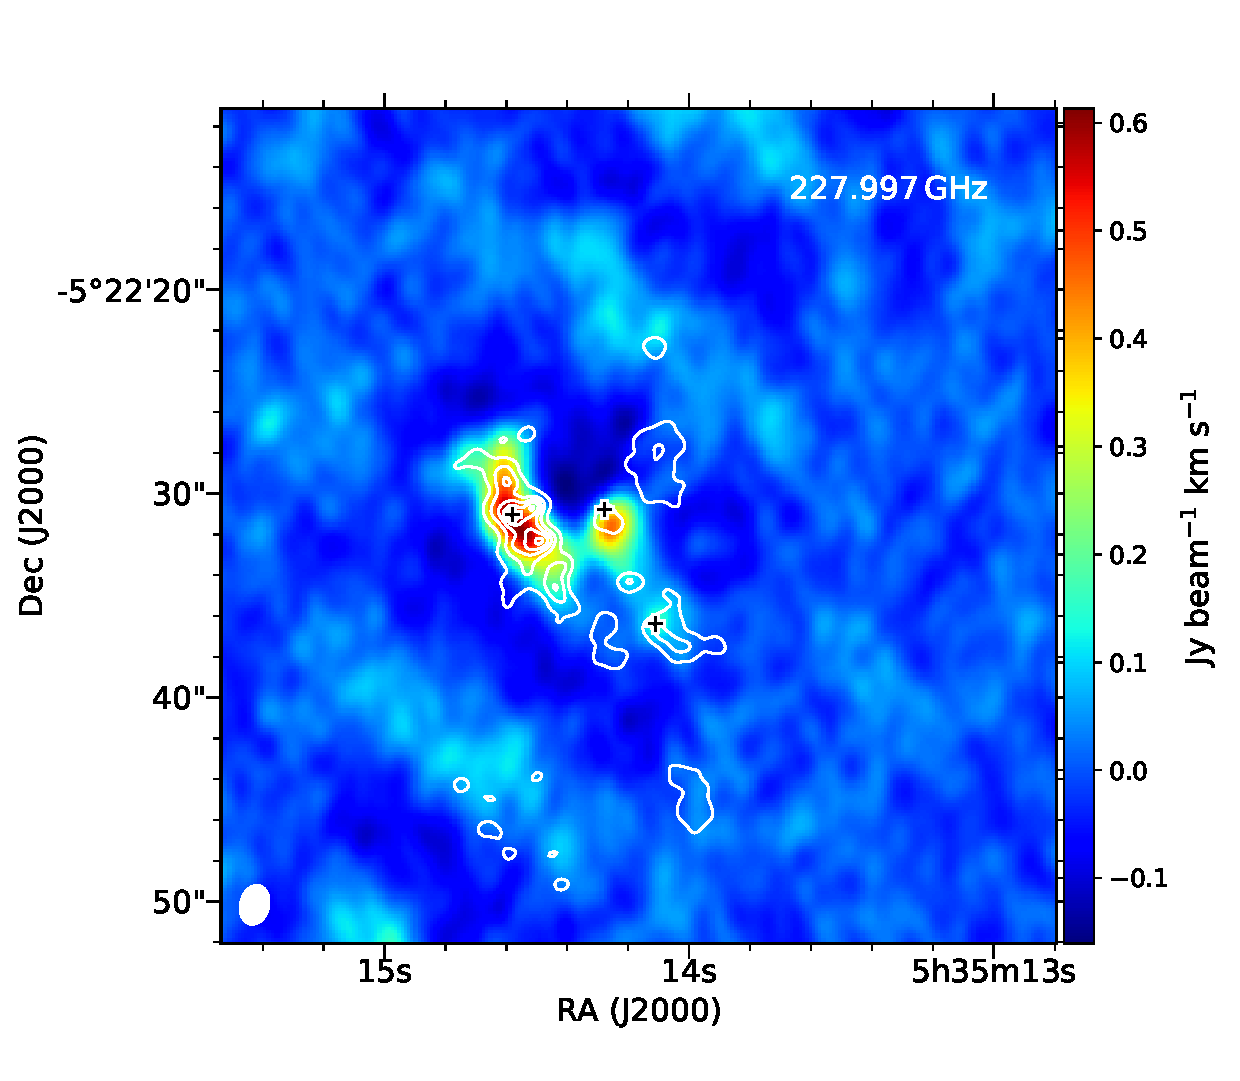
\includegraphics[width=0.98\textwidth]{OrionKL/mom0/227.997SV_mom0_3-7.eps}
%\\(d) 右の図の説明
\end{center}
\end{minipage}
\end{center}
\end{minipage}

%%%% ここから
\begin{minipage}{0.98\textwidth} 
\begin{center}
\begin{minipage}{0.48\textwidth}
\begin{center}
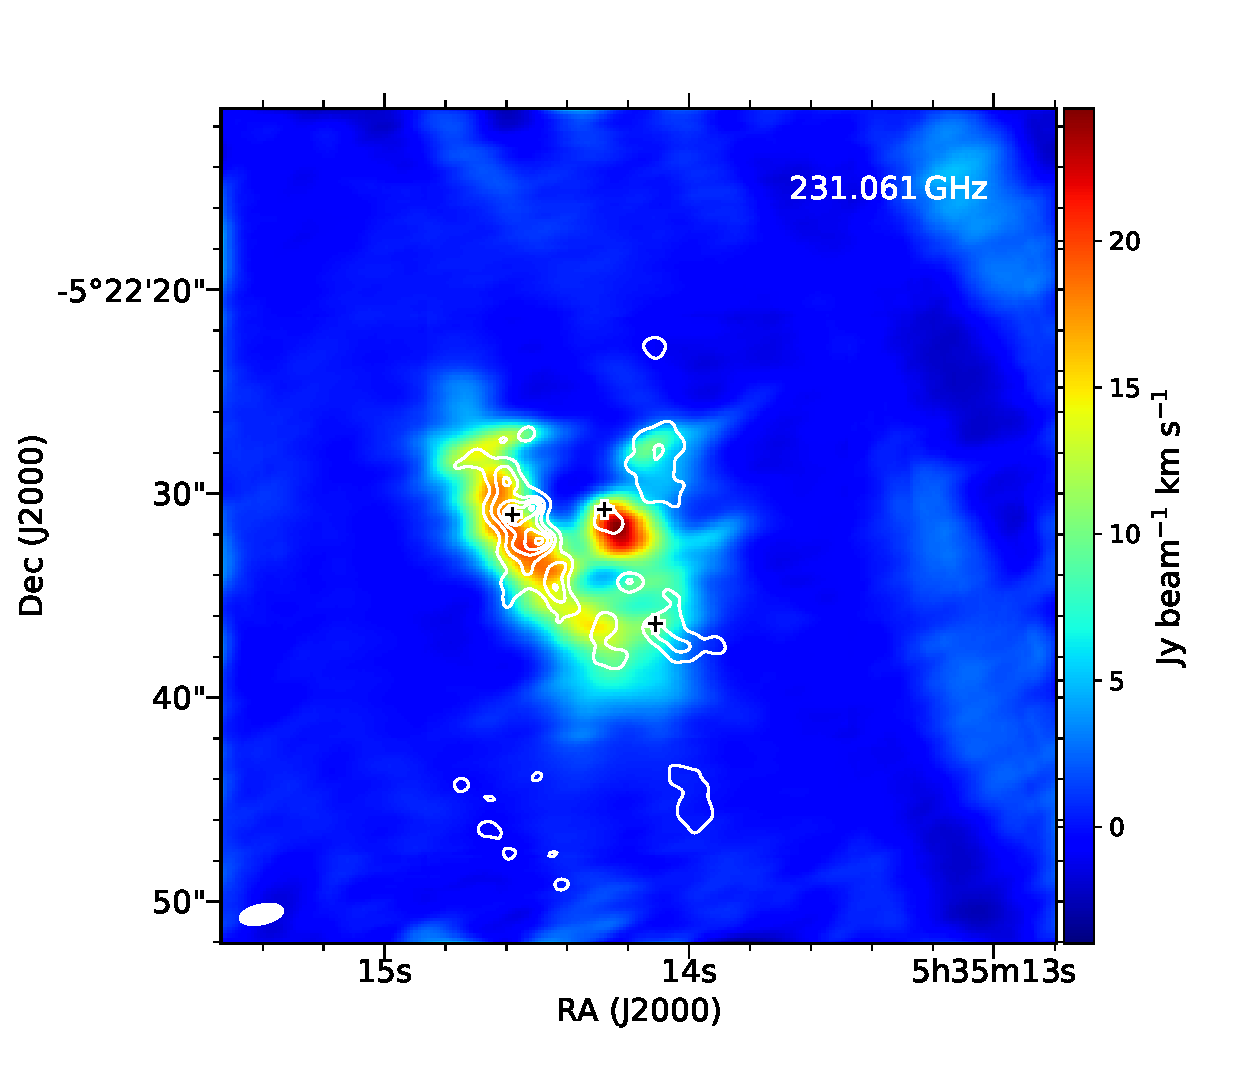
\includegraphics[width=0.98\textwidth]{OrionKL/mom0/231.061mom0_3-7.eps}
%\\(e) 左の図の説明
\end{center}
\end{minipage}
\begin{minipage}{0.48\textwidth}
\begin{center}
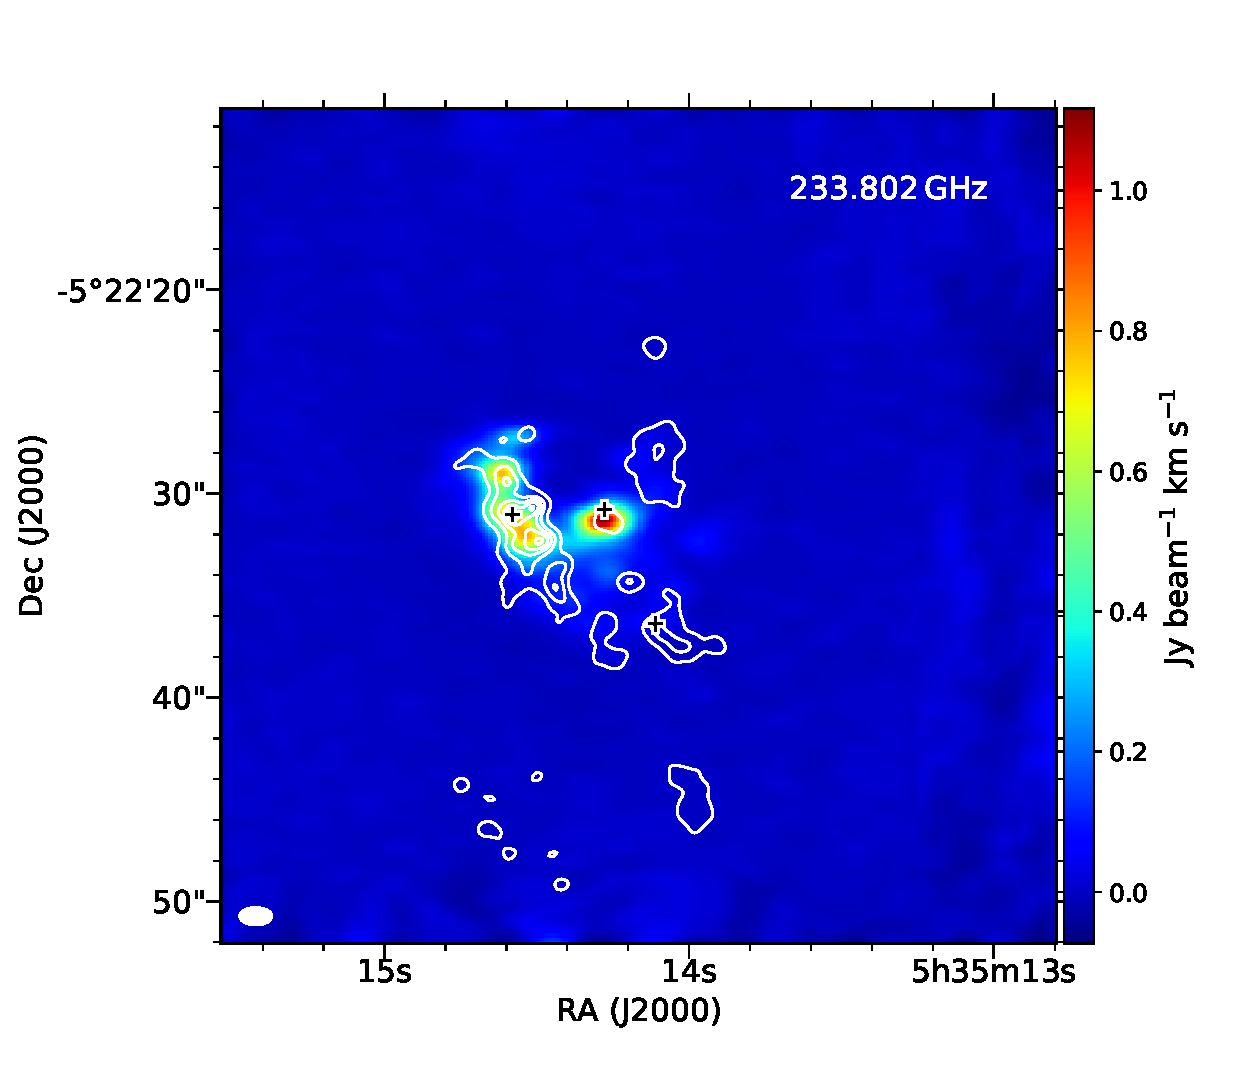
\includegraphics[width=0.98\textwidth]{OrionKL/mom0/233.802mom0_3-7.eps}
%\\(f) 右の図の説明
\end{center}
\end{minipage}
\end{center}
\end{minipage}
%%%% ここまで一組

\caption{(Continued)}
\end{center}
\end{figure}
%%%%%% ここまで

\newpage

%%%%% 積分強度図挿入 %%%%%
\begin{figure}[H] 
\begin{center}

%%%% ここから
\begin{minipage}{0.98\textwidth} 
\begin{center}
\begin{minipage}{0.48\textwidth}
\begin{center}
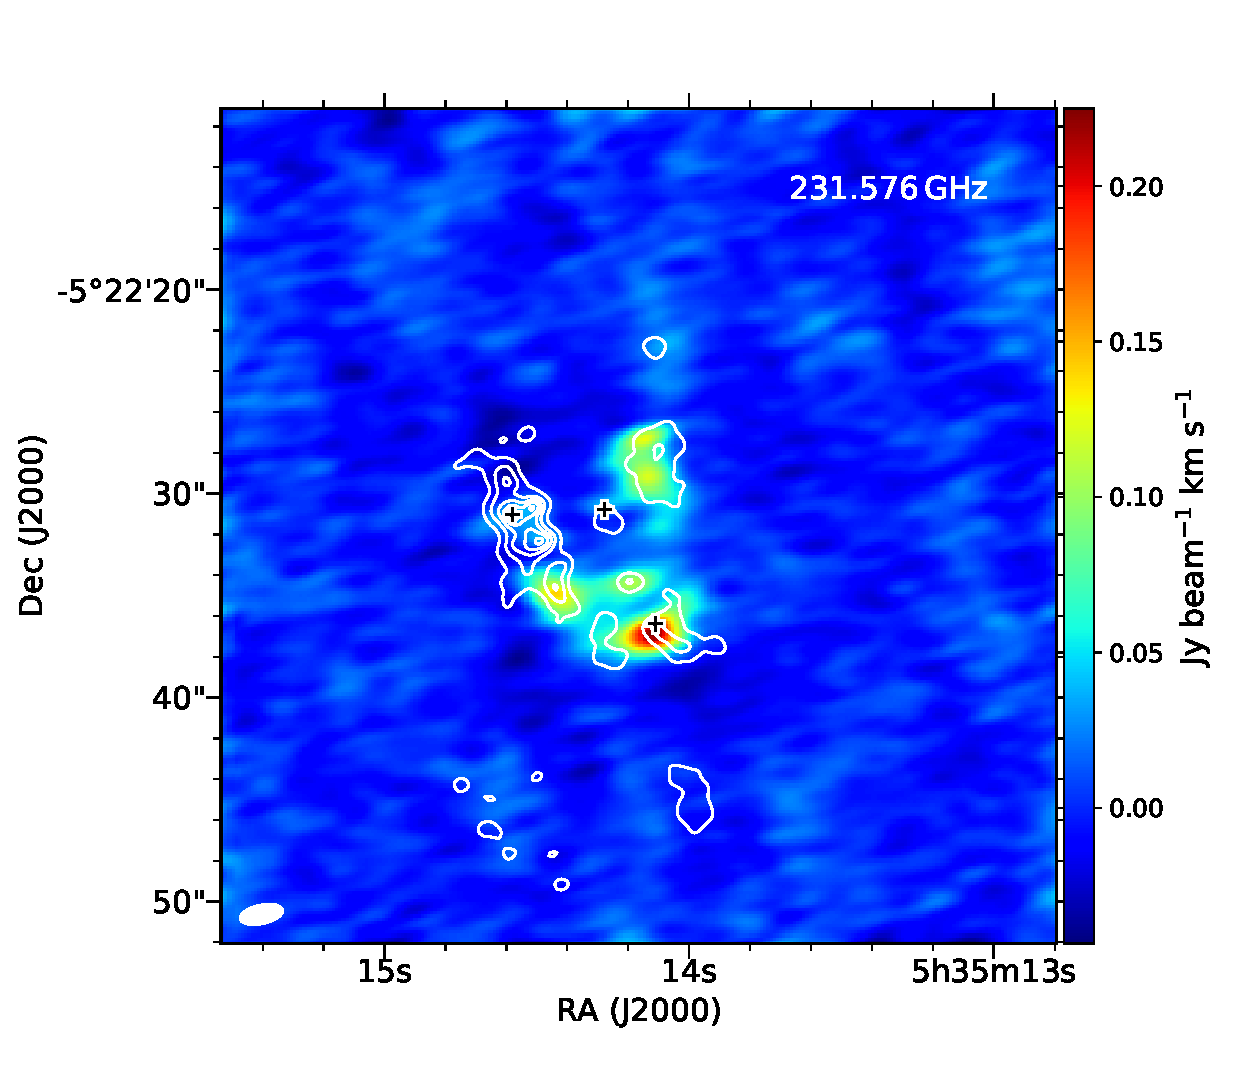
\includegraphics[width=0.98\textwidth]{OrionKL/mom0/231.576mom0_3-7.eps}
%\\(a) 左の図の説明
\end{center}
\end{minipage}
\begin{minipage}{0.48\textwidth}
\begin{center}
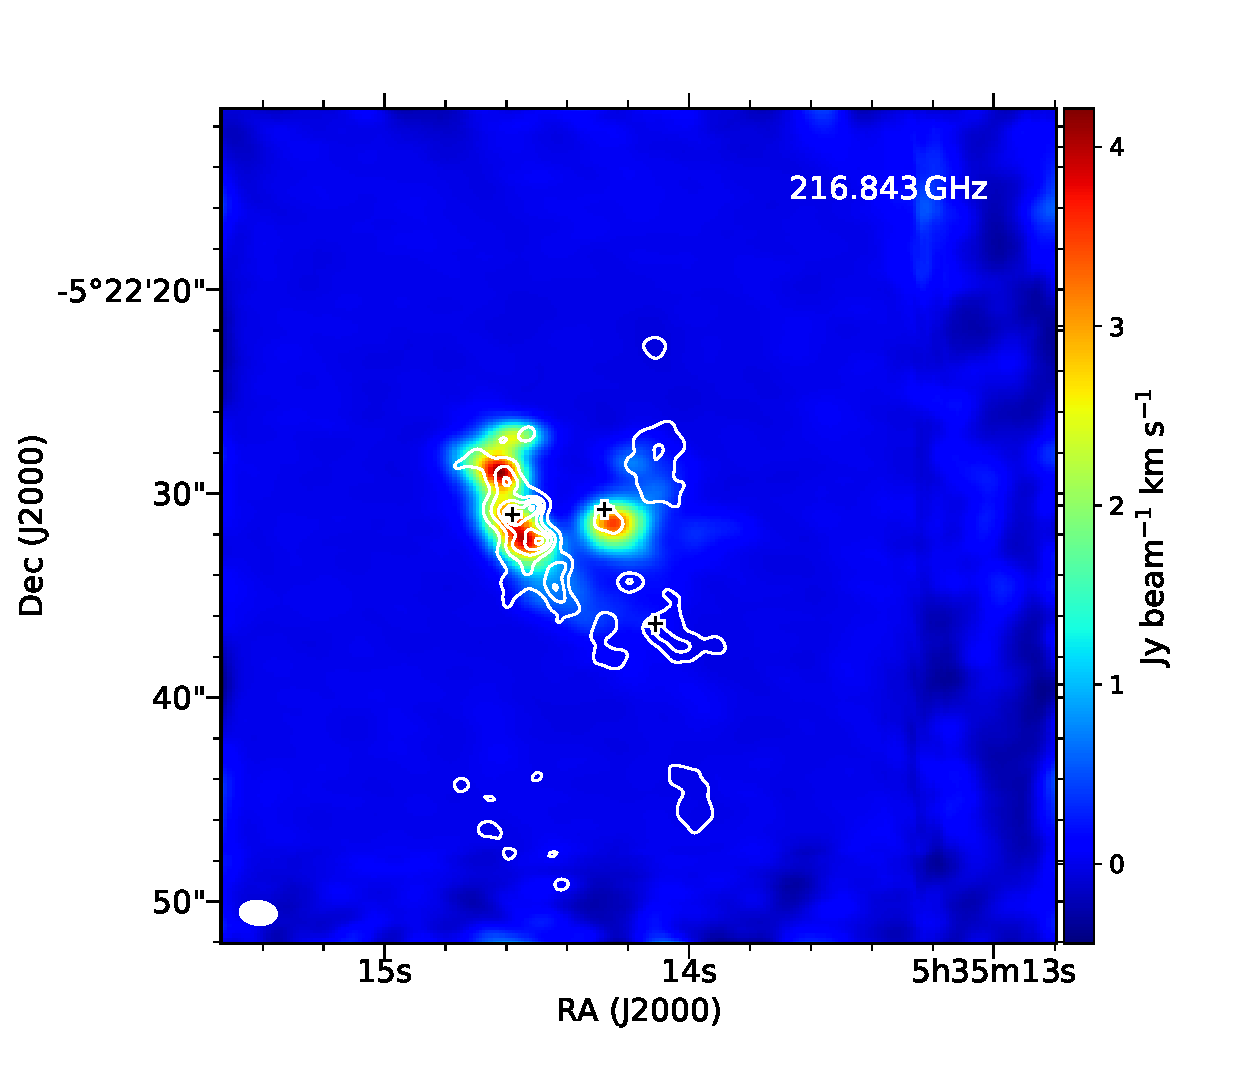
\includegraphics[width=0.98\textwidth]{OrionKL/mom0/216.843mom0_3-7.eps}
%\\(b) 右の図の説明
\end{center}
\end{minipage}
\end{center}
\end{minipage}
%%%% ここまで一組

\begin{minipage}{0.98\textwidth} 
\begin{center}
\begin{minipage}{0.48\textwidth}
\begin{center}
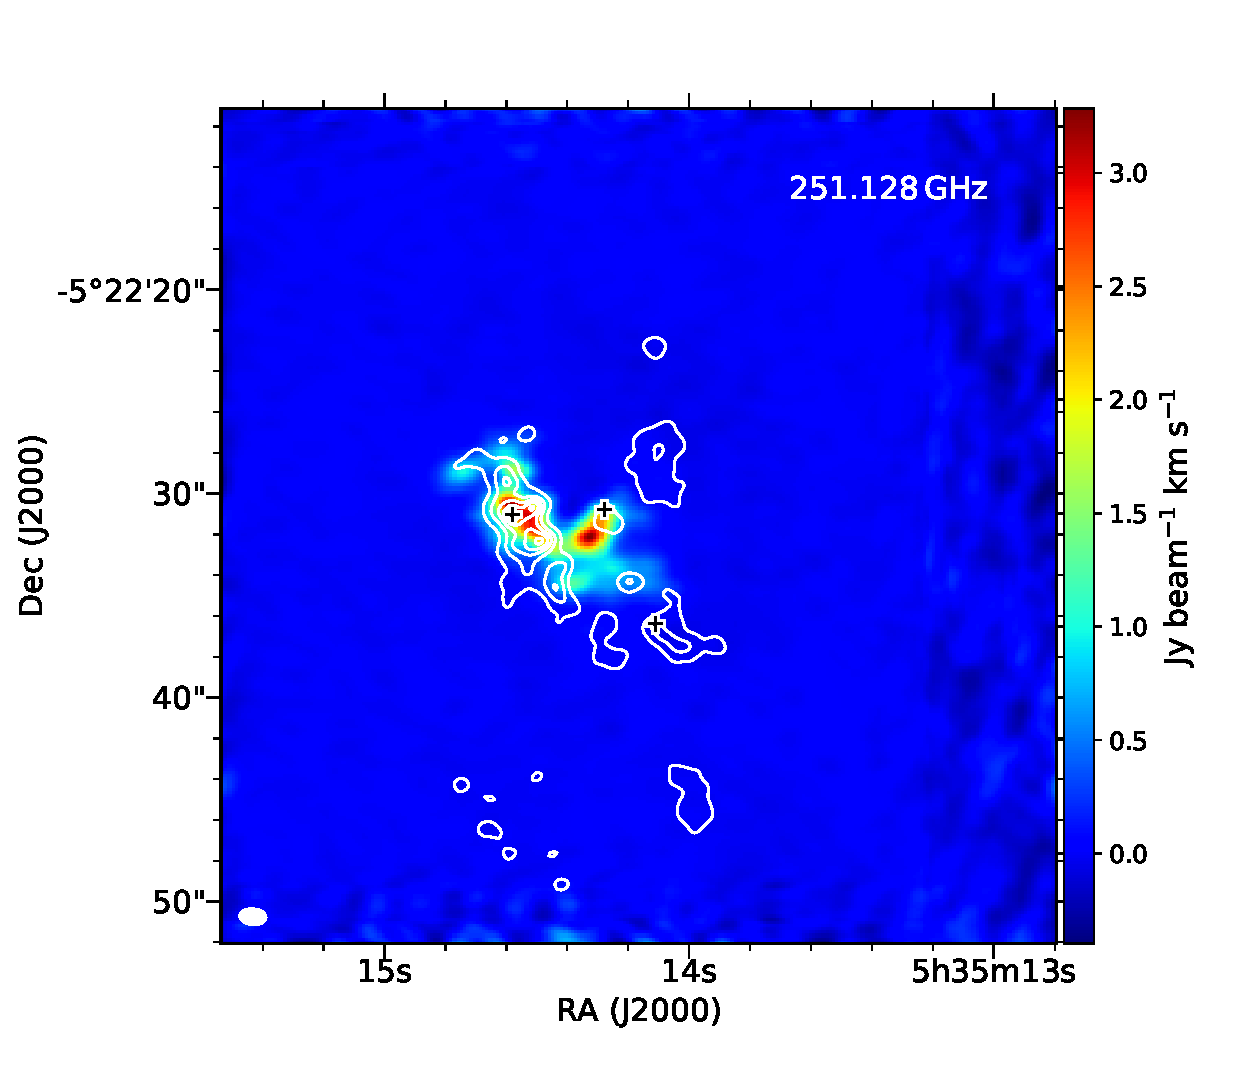
\includegraphics[width=0.98\textwidth]{OrionKL/mom0/251.128mom0_3-7.eps}
%\\(c) 左の図の説明
\end{center}
\end{minipage}
\begin{minipage}{0.48\textwidth}
\begin{center}
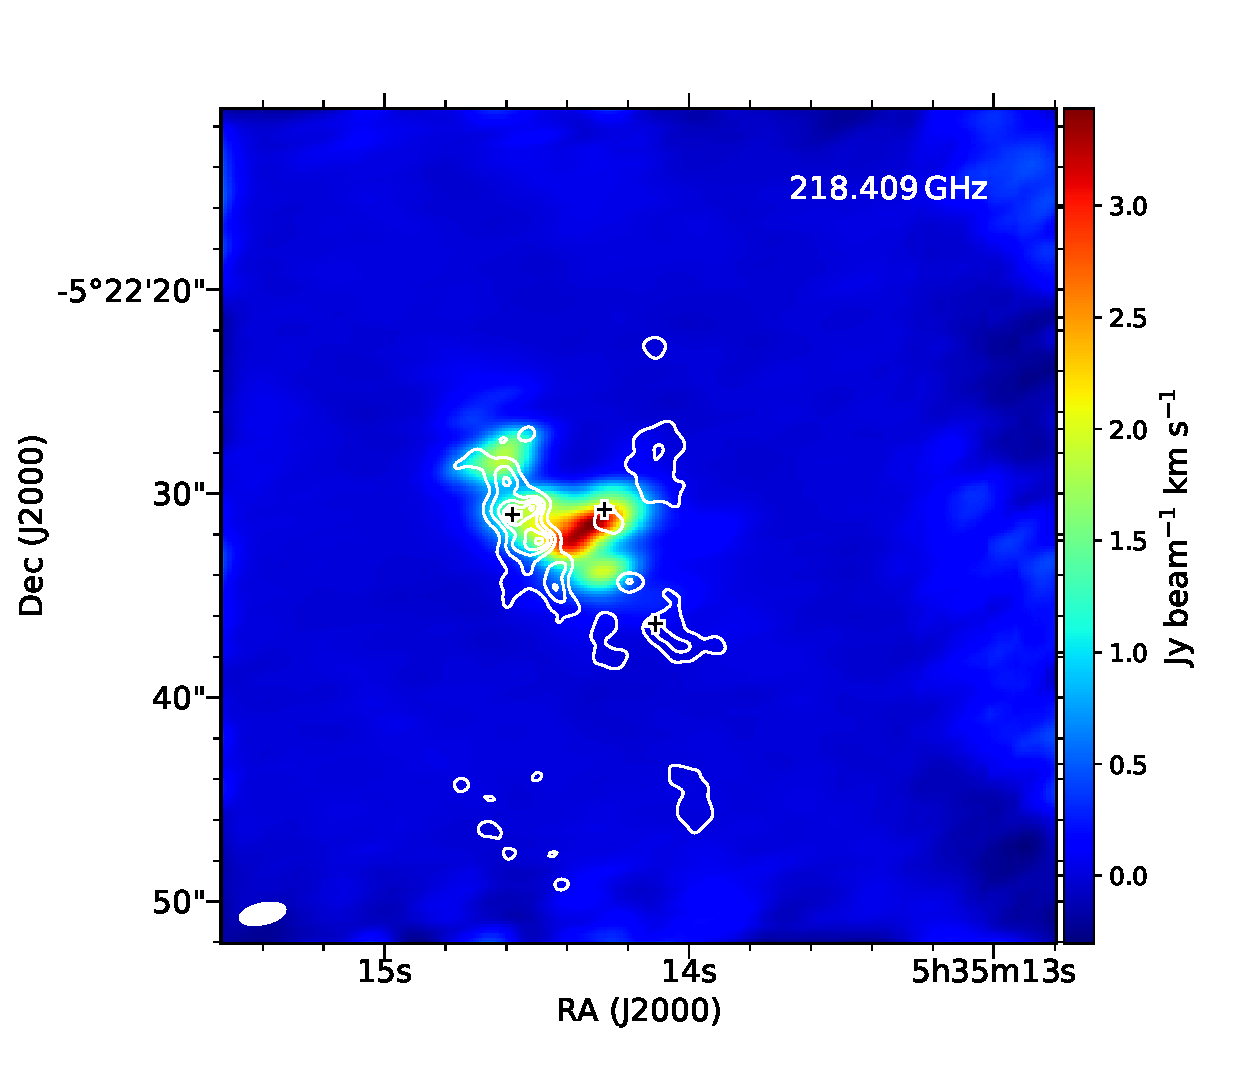
\includegraphics[width=0.98\textwidth]{OrionKL/mom0/218.409mom0_3-7.eps}
%\\(d) 右の図の説明
\end{center}
\end{minipage}
\end{center}
\end{minipage}

%%%% ここから
\begin{minipage}{0.98\textwidth} 
\begin{center}
\begin{minipage}{0.48\textwidth}
\begin{center}
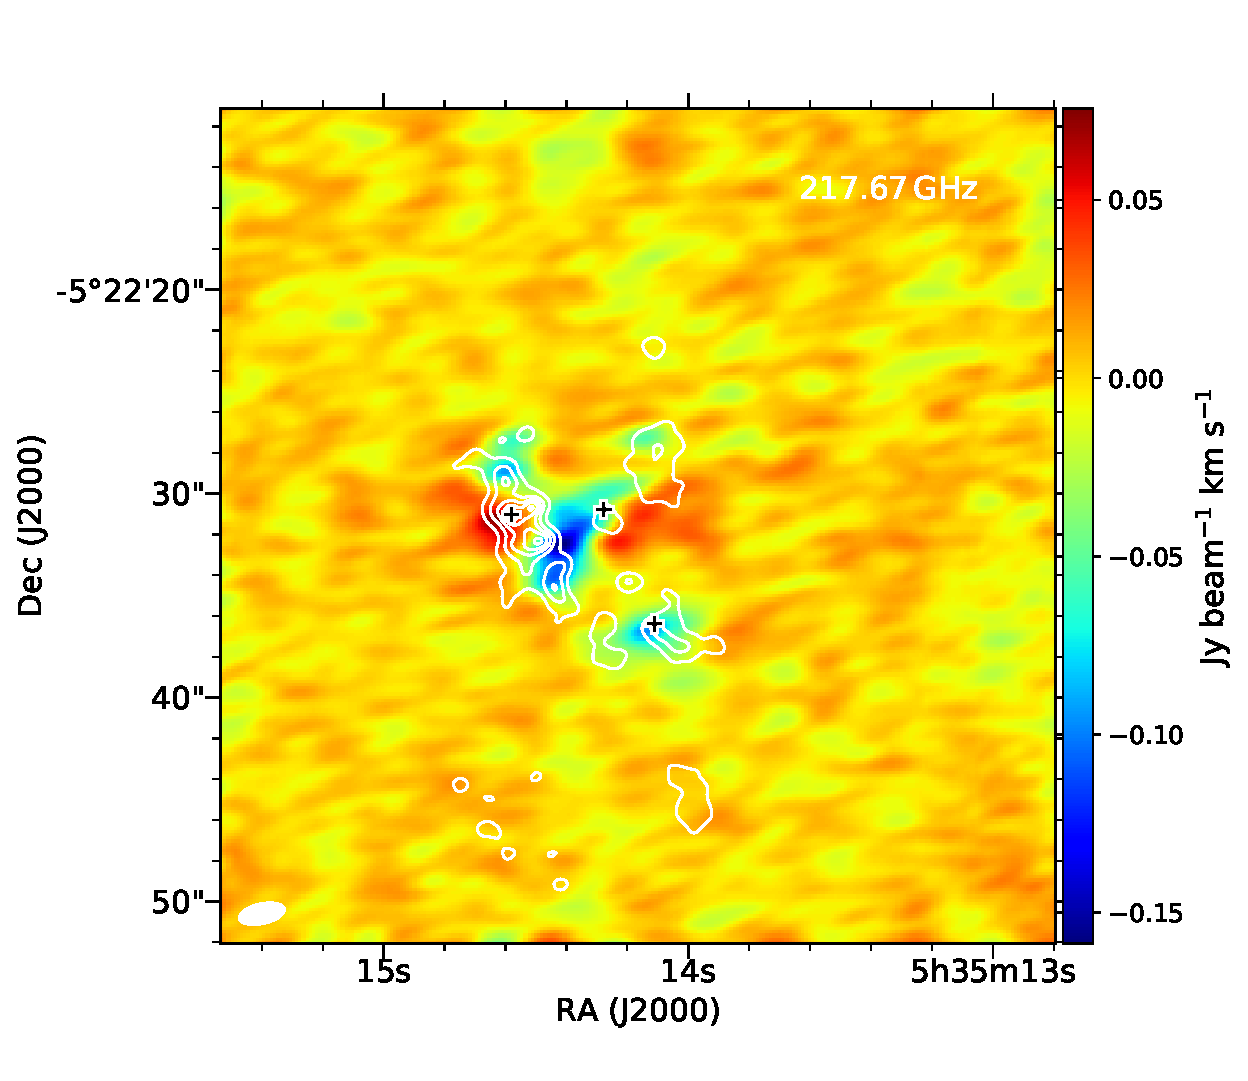
\includegraphics[width=0.98\textwidth]{OrionKL/mom0/217.67mom0_3-7.eps}
%\\(e) 左の図の説明
\end{center}
\end{minipage}
\begin{minipage}{0.48\textwidth}
\begin{center}
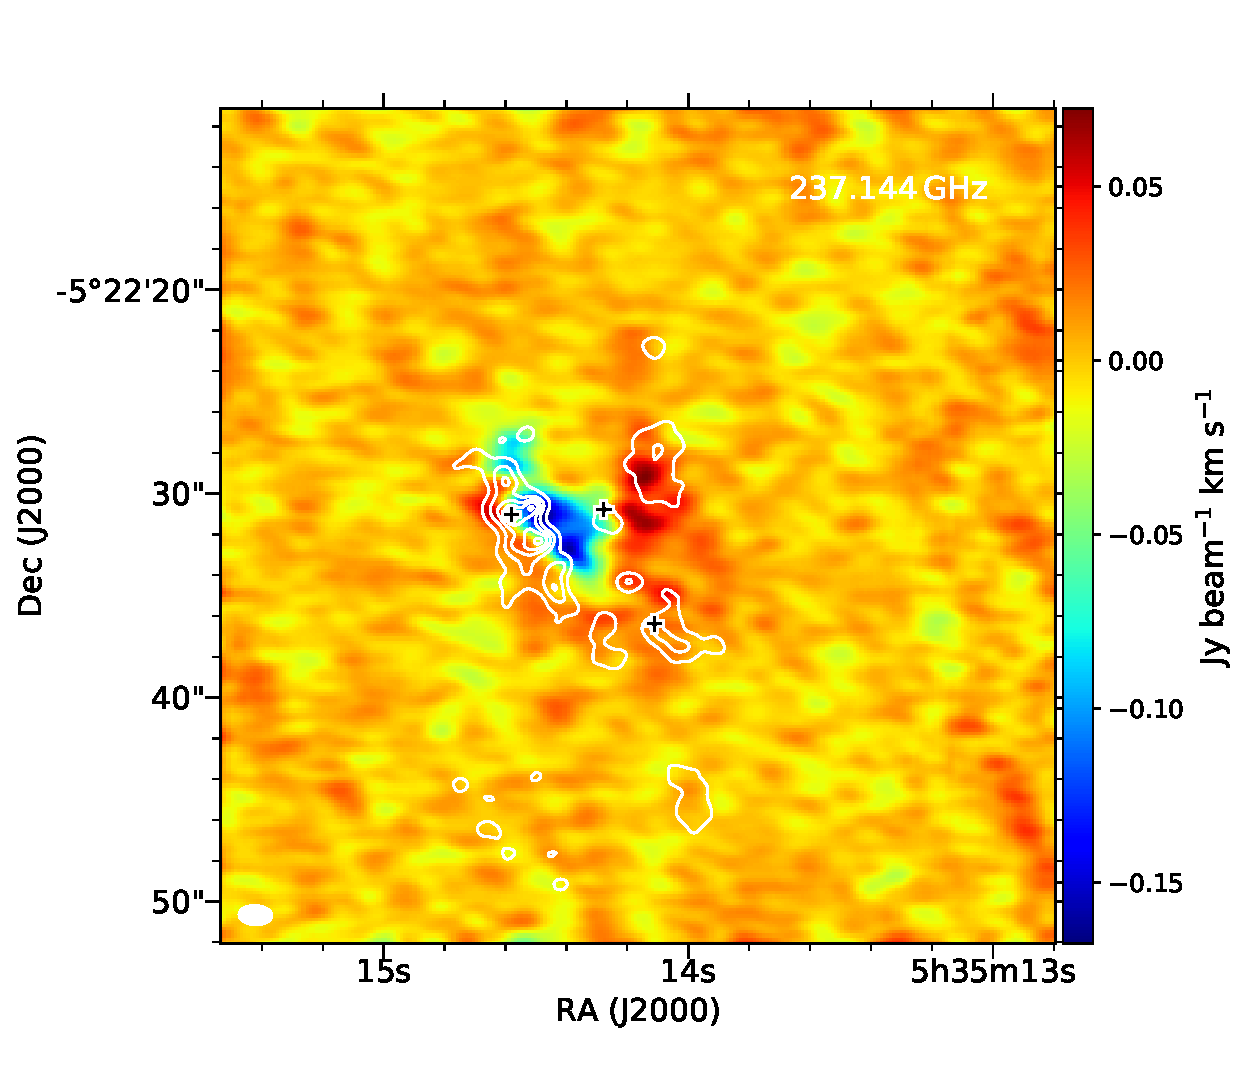
\includegraphics[width=0.98\textwidth]{OrionKL/mom0/237.144mom0_3-7.eps}
%\\(f) 右の図の説明
\end{center}
\end{minipage}
\end{center}
\end{minipage}
%%%% ここまで一組

\caption{(Continued)}
\end{center}
\end{figure}
%%%%%% ここまで

\newpage

\section{Channel maps}

\begin{figure}[htbp]
  \centering
  \includegraphics[width=0.98\textwidth]{OrionKL/chmap/222.846.eps}
  \caption{222.846GHz}
  \label{ap_ch_1}
\end{figure}

\begin{figure}[htbp]
  \centering
  \includegraphics[width=0.98\textwidth]{OrionKL/chmap/227.545.eps}
  \caption{227.545GHz}
  \label{ap_ch_2}
\end{figure}

\begin{figure}[htbp]
  \centering
  \includegraphics[width=0.98\textwidth]{OrionKL/chmap/231.844.eps}
  \caption{231.844GHz}
  \label{ap_ch_3}
\end{figure}

\begin{figure}[htbp]
  \centering
  \includegraphics[width=0.98\textwidth]{OrionKL/chmap/242.625.eps}
  \caption{242.625GHz}
  \label{ap_ch_4}
\end{figure}

\begin{figure}[htbp]
  \centering
  \includegraphics[width=0.98\textwidth]{OrionKL/chmap/231.524.eps}
  \caption{231.524GHz}
  \label{ap_ch_5}
\end{figure}

\begin{figure}[htbp]
  \centering
  \includegraphics[width=0.98\textwidth]{OrionKL/chmap/218.221.eps}
  \caption{218.221GHz}
  \label{ap_ch_6}
\end{figure}

\begin{figure}[htbp]
  \centering
  \includegraphics[width=0.98\textwidth]{OrionKL/chmap/219.151.eps}
  \caption{219.151GHz}
  \label{ap_ch_7}
\end{figure}

\begin{figure}[htbp]
  \centering
  \includegraphics[width=0.98\textwidth]{OrionKL/chmap/227.997.eps}
  \caption{227.997GHz}
  \label{ap_ch_8}
\end{figure}

\begin{figure}[htbp]
  \centering
  \includegraphics[width=0.98\textwidth]{OrionKL/chmap/231.061.eps}
  \caption{231.061GHz}
  \label{ap_ch_9}
\end{figure}

\begin{figure}[htbp]
  \centering
  \includegraphics[width=0.98\textwidth]{OrionKL/chmap/233.802.eps}
  \caption{233.802GHz}
  \label{ap_ch_11}
\end{figure}

\begin{figure}[htbp]
  \centering
  \includegraphics[width=0.98\textwidth]{OrionKL/chmap/231.576.eps}
  \caption{231.576GHz}
  \label{ap_ch_12}
\end{figure}

\begin{figure}[htbp]
  \centering
  \includegraphics[width=0.98\textwidth]{OrionKL/chmap/216.843.eps}
  \caption{216.843GHz}
  \label{ap_ch_13}
\end{figure}


\begin{figure}[htbp]
  \centering
  \includegraphics[width=0.98\textwidth]{OrionKL/chmap/251.128.eps}
  \caption{251.128GHz}
  \label{ap_ch_14}
\end{figure}

\begin{figure}[htbp]
  \centering
  \includegraphics[width=0.98\textwidth]{OrionKL/chmap/218.409.eps}
  \caption{218.409GHz}
  \label{ap_ch_15}
\end{figure}

\begin{figure}[htbp]
  \centering
  \includegraphics[width=0.98\textwidth]{OrionKL/chmap/217.67.eps}
  \caption{217.670GHz}
  \label{ap_ch_16}
\end{figure}

\begin{figure}[htbp]
  \centering
  \includegraphics[width=0.98\textwidth]{OrionKL/chmap/237.144.eps}
  \caption{237.144GHz}
  \label{ap_ch_17}
\end{figure}